\label{sec:definicion_problema}

Una noticia es la comunicación de información seleccionada sobre un evento actual que posteriormente es presentado a través de cualquier medio de comunicación existente.\cite{Shirky_2008_Herecomes}

El periodismo es un método de investigación y el estilo literario utilizado en la representación social y cultural de noticias. Sirve el propósito de jugar el papel de una maquinaria de servicio público en la difusión y el análisis de las noticias y de la información. \cite{harcup2004journalism} 
%la integridad periodística está basada en los principios de la verdad, la exactitud y conocimiento de los hechos. Medios periodísticos pueden variar diversamente, a partir de la publicación impresa a la radiodifusión electrónica, y de periódico a los canales de televisión, así como a la web, y a la tecnología digital. 

En el proceso de generación de una noticia, los periodistas son bombardeados con información provenientes de muy diversas fuentes de la cual deben seleccionar y dar forma a la pequeña cantidad (de información) que se convierte finalmente en la noticia. Este proceso sería imposible sin las etapas de selección, redacción, edición, posicionamiento, programación, repetición y de cualquier otro tratamiento adicional de la información para convertirla en noticia. 
Este conjunto de etapas se denomina como proceso de \emph{gatekeeping} (y a sus gestionadores \emph{gatekeeper}). Desde este proceso, se ofrece una imagen del mundo al público receptor de la noticia, por lo cual es de vital importancia para los estudiosos a entender el proceso de \emph{gatekeeping} y su impacto real en la realidad de los receptores.

El \emph{Gatekeeping} es una de las teorías más antiguas proveniente desde las ciencias sociales, adaptada y desarrollada para su uso en el estudio de las noticias desde la década de 1950, enfocándose principalmente tanto en el producto producto final como en la información seleccionada o rechazada en cada etapa.

\begin{figure}[h]
  \centering
    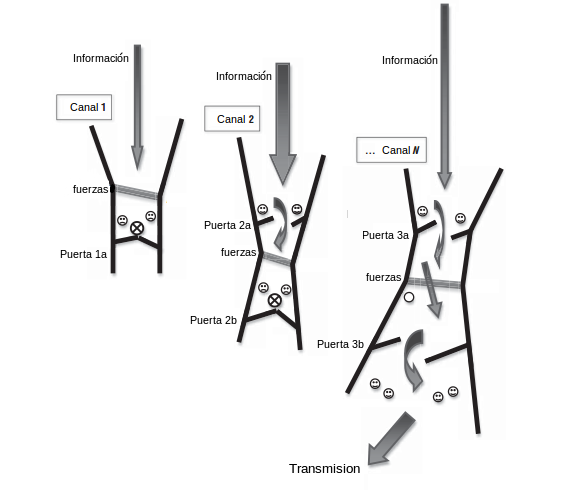
\includegraphics[width=0.6\textwidth]{imgs/gatekeeper.png}
  \caption{Representación del proceso de gatekeeper \cite{wahl2008handbook}}
  \label{fig:gatekeeper}
\end{figure}

La figura \ref{fig:gatekeeper} ilustra un conjunto de elementos que entran en el proceso de \emph{gatekeeping}
No todos los elementos son seleccionados. Algunos hacen su camino en los canales, que a veces se dividen en secciones, cada uno de los cuales se pueden introducir solamente pasando a través de una puerta. Diversas fuerzas facilitan o dificultan el flujo de artículos a través de las diversas puertas, mediante la variación en la magnitud y la dirección del canal. La Figura \ref{fig:gatekeeper} muestra tres canales y muchos elementos de información, pero sólo un elemento se abre camino a través de un canal y se transmite a una o más audiencias. Las fuerzas negativas detienen el progreso de algunos elementos a través de los canales (es importante tener en cuenta que existen fuerzas externas, tanto antes como después de las puertas).

El elemento final que se muestra en la Figura \ref{fig:gatekeeper} como el resultado del proceso de \emph{gatekeeping}, no sólo es el resultado de la selección, sino también el resultado de muchas otras fuerzas, ya que pasa a través de los diversos canales , secciones y puertas. Dos elementos importantes están ocultos: El \emph{gatekeeper} controla si la información pasa a través del canal y controla el resultado final. Cabe señalar que los \emph{gatekeeper} toman muchas formas (ejemplo: personas, códigos profesionales de conducta, políticas de la empresa, los algoritmos informáticos, etc) y todos toman decisiones, pero con distintos grados de autonomía. La autonomía varía desde caprichos idiosincrásicos de un individuo a conjuntos de reglas inquebrantables interpretados por algún algoritmo de un computador.

Las flechas varían en tamaño para indicar cómo los artículos cambian a medida que pasan a través de las diversas puertas o barreras.
El elemento listo para ser transmitido es el resultado de muchas influencias y no siempre se parece al artículo original.

\section{Visiones referente al \emph{gatekeeping}}

Existen diversos análisis y críticas respecto al efecto y real impacto del proceso de \emph{gatekeeping} en la generación de una noticia.

White\cite{white} refiriéndose al proceso lo calificó de \"muy subjetivo\" puesto que las diversas etapas dependen de juicios de valor basados en el conjunto propio de experiencias, actitudes y expectativas del \emph{gatekeeper}. En investigaciones posteriores White sostiene que la selectividad de los periodistas es la principal fuente de ``sesgo" de las noticias gatillado, entre otras cosas, por la necesidad de reducir una multitud de acontecimientos ocurridos en el mundo real a un número modesto, en un tiempo reducido. 
%( 1950, p.386 )
%\footnote{White, D. M. (1950). The gate keeper: A case study in the selection of news. Journalism Quarterly, 27, 383–390}

Aunque no es un estudio de \emph{gatekeeping} en sí mismo, La investigación de Warren Breed de control social en la sala de redacción \cite{breed1955social} aporta interesante componentes para el análisis. Breed, en cierto sentido, identificó a los editores de los periódicos como los \emph{gatekeeper} de facto que operan a través de medios indirectos para asegurar que sólo las noticias en consonancia con la política de la organización sean las generadas. Breed agrega ``Las políticas de noticias podrían modificar o enterrar un evento y de esta manera denegar una información importante a la ciudadanía".

%Although not a “gatekeeping” study as such, Warren Breed’s (1955) research on social control in the newsroom is a close contemporary of White’s and often mentioned together. In “Social control in the newsroom: A functional analysis,” Breed—also a former newspaper reporter— interviewed a sample of newsmen at medium-sized newspapers to determine how they discerned the appropriate way to handle their story selection. Breed, in a sense, identified newspaper pub-
%lishers as the de facto gatekeepers who operate through indirect means to ensure that only news consistent with organizational policy gets through. The relevant gatekeeping issue for Breed was that “policy news may be slanted or buried so that some important information is denied the citizenry” (p. 193).

La contribución de Breed fue mostrar cómo el \emph{gatekeeper} más importante puede no ser necesariamente quien esta relacionado más directamente con la selección, puede residir en otro lugar, dentro de los niveles más influyentes de la organización. Si la noticia es lo que el periodista dice que es, la subjetividad del \emph{gatekeeper} parece problematizar profundamente el proceso de información. Reese y Ballinger en \cite{13213947} argumentan que la razón radica en la expectativa de que actúe adecuadamente en nombre de la comunidad, \emph{el gatekeeper} ``ve a ella (a pesar de que nunca sea consciente de ello) que la comunidad oirá como un hecho único aquellos eventos que el periodista , como representante de su cultura, cree que es verdad". Al igual que White, Breed señala que el proceso \emph{gatekeeping} podría funcionar cumpliendo las expectativas de la comunidad a través de los códigos periodísticos y otras orientaciones, fuera de la influencia indebida de los editores. De acuerdo con estos puntos de vista, mientras los \emph{gatekeeper} se mantengan fieles representantes de la cultura, la sociedad no tiene por qué temer sus decisiones.

%Breed’s contribution was to show how the most important gatekeeper may not be the one who is most immediately involved in the selection, but may reside elsewhere within more influential levels of the organization. If news is what the journalist says it is, the subjectivity of the gatekeeper would seem to profoundly problematize the news process, and yet the field was slow to follow up on this key insight. Reese and Ballinger (2001) argue that the reason lay in the expectation that acting adequately on behalf of the community, the gatekeeper “sees to it (even though he may never be consciously aware of it) that the community shall hear as a fact only those events which the newsman, as the representative of his culture, believes to be true” (White, 1950, p. 390). Like White, Breed implied (as did subsequent interpretations by field synthesizers) that the gatekeeping process could work to the satisfaction of the community via journalistic codes and other guidance, were the undue influence of publishers to be curtailed. According to these views, then, as long as gatekeepers remained faithful cultural representatives, the society need not fear their decisions.

Herbert Gans en \cite{gans1979deciding} identificó las fuentes de poder dentro de la organización periodística y los incentivos que tienen los periodistas para cumplir con las normas del grupo y seguir las consideraciones prácticas. Gans señala que la construcción de la noticia no está principalmente en el periodista o en el editor (o en el editor de ciertos límites) sino en el proceso por el cual todas las partes, las rutinas y las disposiciones de la organización se dedican a la creación de noticias. Reduciendo la responsabilidad directa respecto a la distorsión de individual del periodista.

Para Gans, el proceso de \emph{gatekeeping} es el proceso de solución de los problemas relacionados con el envasado del flujo diario de los acontecimientos, en un producto comercial para el público. Para solucionarlo, los periodistas utilizan ``consideraciones" para ayudar en el proceso, que debe ser aplicables sin demasiada deliberación, éstas deben ayudar a evitar la incertidumbre excesiva, ser flexibles, fácilmente racionalizadas o explicables a los demás y eficientes, garantizando los mejores resultados con el menor esfuerzo. La ecuación de prensa se basa en la eficiencia y el poder, que están estrechamente conectados.

Lewin \cite{lewin1951field} plantea que los individuos debe entenderse en el contexto de cuatro sistemas: un microsistema (contexto inmediato), mesosistema (nexo de contextos inmediatos), exosistema ( instituciones externas ) y macrosistema (cultura o sistema social). Estos cuatro niveles aplicados a la redacción de una noticia incluyen el nivel individual periodista, el nivel de las rutinas o las prácticas de periodismo, el nivel de organización, el nivel de los medios de comunicación y el nivel del sistema social. Lewin sostuvo además que en todos los niveles existen diversas fuerzas las cuales determinan cuales elementos se convierten en noticias y cuales no, limitando la autonomía de los \emph{gatekeeper} y dando forma a las noticias de manera consistente.

%A pesar de que no existen investigaciones sobre la naturaleza de estas fuerzas, aparentent varían dependiendo del nivel considerado. A nivel individual, por ejemplo, la investigación ha demostrado que no todos la toma de decisiones es impulsado por la reflexión consciente - que puede dar como resultado la misma facilidad de factores subconscientes, tales como una disponibilidad o heurística de la representatividad ( Nisbett y Ross, 1980 ). En el nivel de sistema social, por su parte , instituciones sociales crean " limitaciones y oportunidades a los que los medios de comunicación y los actores responden " ( Hallin y Mancini, 2004 , p. 296 ). Estas limitaciones y oportunidades que emergen basan en el desarrollo contemporáneo de las instituciones económicas , políticas y medios de comunicación. Contenido de las noticias es similar en un sistema social, porque los actores responden racionalmente a las mismas limitaciones y oportunidades. En la medida en que el entorno institucional puede producir más de un camino racional , podríamos esperar variaciones incluso entre actores racionales.

Walter Lippman, en su libro \emph{Public Opinion} \cite{lippmann1922public} señala taxativamente que \"el papel de la prensa es el de ser en cierto modo servidor y guardián de las instituciones\" y sugiere que las fuerzas planteadas por Lewin se relacionan con este \"rol\" que juegan los procesos de comunicación y los medios. Este proceso según Laswell en \cite{Lasswell2007Structure} afirma se realiza tres funciones: 
\begin{enumerate}
\item Vigilancia del entorno, revelando amenazas y oportunidades que afecten a la posición de valor de la comunidad y de las partes que la componen.
\item Correlación de los componentes de la sociedad en cuanto a dar una respuesta al entorno. 
\item Transmisión del legado social. 
\end{enumerate}
De una forma esquemática ha sido descrito este triple papel de esta otra manera: vigilancia, foro para la discusión y escuela.\cite{informacionsociedad} 

Smith \cite{tedsmith} explica precisamente una de estas tres funciones capitales, la de vigilancia del entono, a la que algún retórico vino a describir con una metáfora: la tarea del ``perro guardián suponía que cada periódico atacaría y defendería desde una posición determinada, y que del conflicto entre todos, surgiría la verdad (...) Hoy en día, por el contrario, la prensa abarca muy numerosos medios de noticias, tanto impresos como electrónicos. En esta categoría se incluye un escogido y selecto puñado de diarios y semanarios, los servicios cablegráficos, las noticias de redes radiofónicos y, sobretodo, las principales cadenas de televisión. En virtud de sus dimensiones y prominencia, son estos pocos medios de élite los que establecen el tono de los programas de cobertura para la mayor parte de la prensa" señalando además que los periodistas, en cuanto críticos sociales y políticos, no desempeñan correctamente la labor encomendada a causa de carencias estructurales en estos cuatro aspectos: 

\begin{enumerate}
\item El ejercicio periodístico es básicamente una actividad de escaso rigor intelectual y con marcada tendencia a la simplificación. 
\item Los periodistas suelen carecer de conocimientos técnicos adecuados para la mayor parte de las cuestiones complejas de la vida actual.
\item El trabajo periodístico se ejecuta sin la reflexión y el sosiego que son deseables en una adecuada labor crítica. 
\item Es evidente la falta de una actitud juiciosa y equilibrada en la mayor parte de los periodistas, que renuncian a hacer un
balance de los datos positivos y negativos para reducirse únicamente a una esquemática y simplificadora enumeración de defectos aparentes sin analizar las causas.
\end{enumerate}

Jean-François en su conocido libro 'El conocimiento inútil' \cite{revel1990conocimiento} crítica en todos los casos, y no solamente cuando se ataca al gobierno, en que la prensa se considera como un magistrado: ``la generación de noticias debe resultar de la información correctamente establecida, y no dirigir la elección de esa información a impulsos de un prejuicio selectivo, que metamorfosea la despiadada ferocidad para con unos en indulgencia sin límites para con otros". Según el análisis de este autor ``lo que predomina desgraciadamente en muchos periódicos de nuestro entorno sociocultural es el dirigismo apriorista en contra del poder, la predisposición condenatoria contra los actos emanados de las instituciones gubernamentales".

Real, Agudiez, Príncipe en \cite{ESMPESMP0707110189A} señalan que ``El Periodismo parece no haber cumplido con su parte del \emph{contrato social}. Los ciudadanos se sienten descontentos y defraudados por unos profesionales y unas empresas que parecen haber modificado los fines que un día iluminaron su quehacer comunitario. El diario on–line Periodista Digital justifica las razones que han motivado el repudio de las audiencias: (...) los ciudadanos están rechazando a los viejos medios de comunicación, a los que considera comprados y mediatizados. Como consecuencia, esos medios tradicionales pierden cada día credibilidad y audiencia'. De hecho, las investigaciones sociológicas revelan que los consumidores de información están perdiendo la confianza en los periodistas y en los medios a pasos agigantados, porque los consideran al servicio no de la ciudadanía sino del poder y de sus intereses políticos y económicos".

Con una visión contraria Lorenzo Gomis en \cite{gomis1991teor} ha desarrollado la siguiente idea: los medios de comunicación y los periodistas no sienten interés por los problemas derivados de las posibles repercusiones de sus mensajes. ``La mayor influencia que se ejerce en los medios no es a través de los comentarios, sino de los mismos hechos. Y por lo tanto influye quien aporta el hecho, ya sea el interesado en el hecho que le favorece, o ya sea el interesado que perjudica a su adversario. Los medios son en definitiva la escena donde se luchan los productores de hechos para influir en la gente, mientras que los que controlan el medio sólo se interesan relativamente en esa pugna (...) Los más interesados en influir en los medios no son ni los que los poseen ni los que trabajan en ellos. Curiosa situación".
Para este autor el accionar de los \emph{gatekeeper} no tiene motivaciones otras que no sean técnicas: ``Los seleccionadores o gatekeepers no ponderan la influencia potencial de los hechos en cuanto a sus efectos políticos o sociales, sino que consideran únicamente su condición técnica de noticia y, en caso de duda, es sumamente probable que la noticia quedará sin publicar".

A finales de la década de los noventa surgió una alternativa a esa visión de los medios de prensa como una entidad que resguardaba de forma neutral los intereses de los ciudadanos, que implicaba a los mismos ciudadanos, esto posibilitado -entre otras cosas- por la irrupción de Internet y las profundas transformaciones que supone en la información periodística y las vías de acceso a la información.

Las nuevas tecnologías brindan diferentes oportunidades para la incorporación de las inquietudes de los ciudadanos en los discursos
dominantes de los medios mediante su participación directa en la producción informativa. Un nuevo escenario donde los pasivos y silenciosos ciudadanos se convierten en potenciales productores de información.

La adaptación de los medios de comunicación a este nuevo escenario, prevé una comunicación multidireccional entre medio y audiencia. En ese sentido, los medios de comunicación intentan consolidar mecanismos de participación en sus medios digitales. No obstante, tal y como señala Hermida en \cite{doi17512781003640703} en una investigación en que examina las oportunidades que el usuario tiene de participar en el proceso periodístico (participación, acceso, selección, edición y distribución), los medios de comunicación suelen ofrecer herramientas de participación similares entre sí y raras veces permiten que la audiencia participe del \emph{gatekeeping}. “Nuestro estudio indica que la selección, o filtro, es el proceso de \emph{gatekeeping} más cerrado para los usuarios, y creemos que seguirá siéndolo” \cite{doi17512781003640703}%pagina21

Shayne Bowman y Chris Willis presentan en su informe ``\emph{We Media}" \cite{wethemedia} las valiosas ventajas de incorporar a los ciudadanos en la producción de información:
\begin{enumerate}
\item La posibilidad para los lectores de que hagan comentarios.
\item La función de un filtro de noticias para noticias encontradas en la web a través de enlaces.
\item El control de exactitud en la información publicada.
\item El enriquecimiento de fuentes e ideas para periodistas gracias a las sugerencias e historias presentadas por los lectores.
\item La posibilidad para que los periodistas le pidan sugerencias y correcciones al público.
\end{enumerate}
%(2003) 

Existe una gran cantidad de situaciones en las que los ciudadanos han colaborado con el envío de informaciones, imágenes y vídeos sobre un acontecimiento. Contribuyendo a comunicar un suceso desde su propia perspectiva. 
A ese fenómeno se le reconoce como periodismo ciudadano, periodismo de fuente abierta o periodismo en red, que son sinónimos de lo que Bowman y Willis denominan periodismo participativo en Internet. En \cite{wethemedia} lo definen como “el acto de un ciudadano o grupo de ciudadanos que juegan un papel activo en el proceso de colectar, reportar, analizar y diseminar información”, que con frecuencia ocurre en un medio social y colaborativo. %(Bowman y Willis, 2003, p. 9).

En este proceso, el usuario no está solo, hay una comunidad de internautas que se reúnen para producir de forma colaborativa. En este caso, no existen límites geográficos, lo que cuenta es el conocimiento, el trabajo creativo y el deseo de colaborar.
Esa comunidad de usuarios también se dedica a filtrar contenidos y recomendarlos a sus contactos en la Red. A este proceso Bruns en \cite{quteprints189} denomina \emph{gatewatching}. A diferencia del proceso de \emph{gatekeeping} no se busca seleccionar la información, sino de dar facilidades y atajos de lectura.

Los formatos más comunes para la participación del internauta en los medios de comunicación incluyen: Blogs de ciudadanos, envío de fotografías y vídeos, envío de textos, entrevistas colectivas, comentarios, ranking de contenidos elaborados de acuerdo con los votos de usuarios, foros, blogs de periodistas, encuestas y redes sociales como Facebook y Twitter \cite{doi17512781003640703} %(Hermida, 2010).

Arriagada y Navia en \cite{intermedio2013} plantean que la irrupción de la tecnología no solo amplió las posibilidades de producción y acceso del usuario sino también modificó las relaciones de poder e influencia entre los medios, las audiencias y los grupos políticos, empoderando a los ciudadanos permitiendo el desarrollo de interacciones entre la clase política y la gente de forma independiente del quehacer de los medios. "Si históricamente los medios podían ser considerados como el cuarto poder, en tanto constituían una institución de la sociedad que podía vigilar el comportamiento de la clase gobernante, ahora los propios medios son a su vez vigilados por grupos que, a través de redes sociales online, participan activamente en los debates públicos, y que a menudo presentan niveles de desconfianza relativamente altos hacia las instituciones. En las redes sociales online, estos niveles de desconfianza pueden alcanzar también a los medios. Es más: en la medida que la gente percibe a los medios como parte de la institucionalidad o como representantes de las élites, los crecientes niveles de desconfianza en las instituciones también pueden alcanzarlos."

\section{Twitter y su relación con el periodismo}

Además de red social, Twitter se ha convertido en un sistema de noticias compartidas en línea, que se basa en mensajes cortos, rápidos y frecuentes. Hermida \cite{hermida2010twittering}
%(2010) 
describe este sistema como un medio ambiente que muestra la información en un espacio ocupado por el usuario.
En este sistema, un usuario recibe la información en la periferia de su conciencia, es decir, Twitter no requiere la misma atención cognitiva que un e-mail, por ejemplo. Se refiere a una especie de medio ambiente periodístico que ofrece diversos medios para recopilar, comunicar y compartir noticias e información. 

%En el trabajo periodístico, las redes sociales con plataforma de microblogging, como Twitter, favorecen tanto la difusión instantánea de la información corta (Hermida, 2010) como la movilidad (Silva, 2009). Conforme Silva (2009), Twitter forma parte de los moblogs, que también
%son utilizados como herramientas periodísticas. A la estructura de tecnologías móviles conectadas a Internet por wireless (móviles, smartphones, portátiles, tablets, etc.) que se suele usar durante la cobertura de un evento o suceso, Silva (2009, p. 260) la denomina como un ambiente móvil de producción, “que se vincula directamente al moblog periodístico ampliando las condiciones de movilidad del
%trabajo de campo”.

Debido que es posible el acceso a Twitter desde teléfonos móviles existe una nueva estructura de movilidad al periodismo, tanto en la producción como la difusión de la información, ya que la conectividad de los dispositivos móviles a Internet permite la instauración de la instantaneidad de la noticia. Siendo así, la movilidad puede reconfigurar el trabajo de edición de blogs y la generación de contenidos periodísticos en las redes sociales. 
%(Silva, 2009).
Por su carácter instantáneo, Twitter sirve como plataforma para la realización de la cobertura periodística de eventos, en la cual se elabora un tipo de crónica de última hora o flash , pero en orden cronológico inverso. El flash corresponde a una información de última hora, de elevada importancia y gran impacto informativo. 
Suele ser un texto conciso en que se priorizan los aspectos más relevantes del acontecimiento. De acuerdo con Salaverría , el flash es solo un arranque de una cadena de informaciones, que resultará en un texto más completo que responda a las seis preguntas clásicas de toda noticia. El flash se ha ido convirtiendo en notas informativas cortas, limitadas a 140 caracteres (límite establecido por los servicios de mensajería instantánea y Twitter).\cite{salaverria2005redaccion}
%(Salaverría, 2005)

Un guía oficial de Twitter para las redacciones fue lanzado en junio de 2011, tal vez a raíz de la iniciativa de la página para Periodistas en Facebook, lanzada en abril de 2011, en ella se señalaba: \"Twitter es una herramienta de todos los periodistas pueden utilizar para encontrar las fuentes más rápido, contar historias mejor y construir una mayor audiencia para su trabajo\".
